\documentclass{article}

\usepackage{tikz}
\usepackage{graphicx}
\usetikzlibrary{arrows.meta,decorations.pathreplacing}

\begin{document}
	
	\begin{figure}[ht]
		\centering
		
		\resizebox{\textwidth}{!}{%
			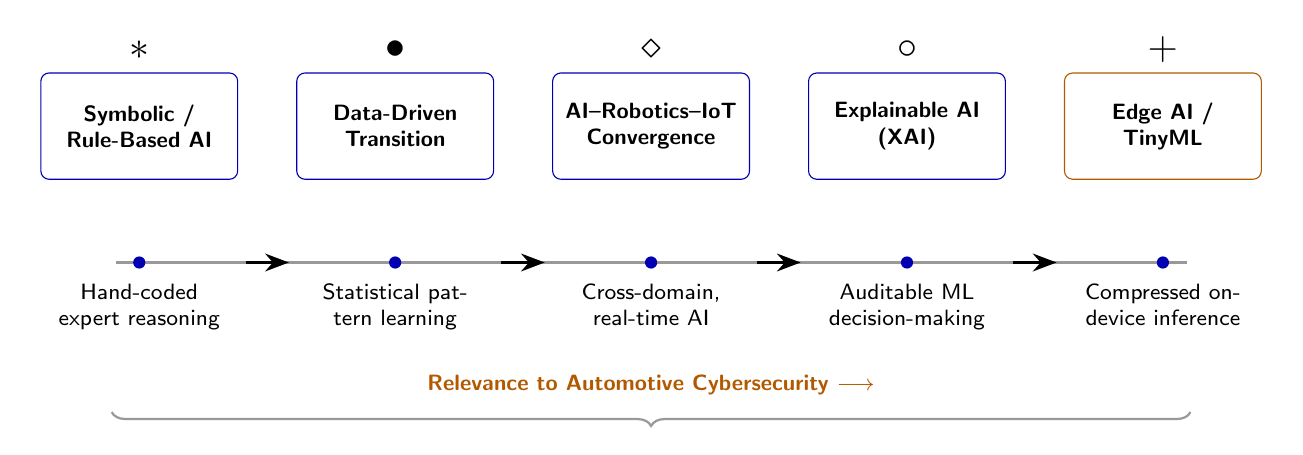
\begin{tikzpicture}[
				box/.style={
					draw=blue!70!black,
					rounded corners=3pt,
					minimum width=2.5cm,
					minimum height=1.35cm,
					align=center,
					font=\sffamily\bfseries\footnotesize
				},
				accentbox/.style={
					draw=orange!70!black,
					rounded corners=3pt,
					minimum width=2.5cm,
					minimum height=1.35cm,
					align=center,
					font=\sffamily\bfseries\footnotesize
				},
				desc/.style={
					text width=2.6cm,
					align=center,
					font=\sffamily\footnotesize
				},
				arrow/.style={
					-{Stealth[length=3mm]},
					line width=1.2pt
				}
				]
				
				% Timeline
				\draw[line width=1.4pt, gray!80] (-0.3,0) -- (13.3,0);
				
				% Timeline dots
				\foreach \x in {0,3.25,6.5,9.75,13}
				\fill[blue!70!black] (\x,0) circle (2.2pt);
				
				% Main boxes
				\node[box, anchor=south] at (0,1.05)
				{\textbf{Symbolic /}\\\textbf{Rule-Based AI}};
				
				\node[box, anchor=south] at (3.25,1.05)
				{\textbf{Data-Driven}\\\textbf{Transition}};
				
				\node[box, anchor=south] at (6.5,1.05)
				{\textbf{AI--Robotics--IoT}\\\textbf{Convergence}};
				
				\node[box, anchor=south] at (9.75,1.05)
				{\textbf{Explainable AI}\\\textbf{(XAI)}};
				
				\node[accentbox, anchor=south] at (13,1.05)
				{\textbf{Edge AI /}\\\textbf{TinyML}};
				
				% Simple icons
				\node[font=\Large] at (0,2.7) {$\ast$};
				\node[font=\Large] at (3.25,2.7) {$\bullet$};
				\node[font=\Large] at (6.5,2.7) {$\diamond$};
				\node[font=\Large] at (9.75,2.7) {$\circ$};
				\node[font=\Large] at (13,2.7) {$+$};
				
				% Descriptions
				\node[desc, anchor=north] at (0,-0.15)
				{Hand-coded expert reasoning};
				
				\node[desc, anchor=north] at (3.25,-0.15)
				{Statistical pattern learning};
				
				\node[desc, anchor=north] at (6.5,-0.15)
				{Cross-domain, real-time AI};
				
				\node[desc, anchor=north] at (9.75,-0.15)
				{Auditable ML decision-making};
				
				\node[desc, anchor=north] at (13,-0.15)
				{Compressed on-device inference};
				
				% Arrows
				\draw[arrow] (1.35,0) -- (1.9,0);
				\draw[arrow] (4.6,0) -- (5.15,0);
				\draw[arrow] (7.85,0) -- (8.4,0);
				\draw[arrow] (11.1,0) -- (11.65,0);
				
				% Relevance text
				\node[
				font=\sffamily\bfseries\footnotesize,
				text=orange!70!black
				] at (6.5,-1.55)
				{Relevance to Automotive Cybersecurity $\longrightarrow$};
				
				% Brace
				\draw[
				decorate,
				decoration={
					brace,
					amplitude=5pt,
					mirror
				},
				line width=0.8pt,
				gray!80
				] (-0.35,-1.9) -- (13.35,-1.9);
				
			\end{tikzpicture}%
		}
		
		\caption{Evolution of Artificial Intelligence Technologies.}
		\label{fig:ai_evolution}
		
	\end{figure}
	
\end{document}